\chapter{\label{chap:descr}Descrição do Projeto}

\section{Algoritmo}
O algoritmo a ser implementado é o AHTN. Nele são combinados tecnicas de HTN com o algoritmo \textit{minimax game tree search}. 
%algoritmo a ser utilizado \\
%algoritmo de ML a ser agregado

\section{Ambiente}

O ambiente que será utilizado é o MicroRTS.  O jogo MicroRTS foi feito por Santiago Ontañón \cite{ontanon2013combinatorial} para fins acadêmicos, com o intuito de aplicar e desenvolver técnicas de IA e para servir como prova de conceito para as técnicas criadas.  O jogo é uma simplificação do jogo Starcraft\footnote{http://us.battle.net/sc2/pt/}.
A figura \ref{fig:microrts} mostra uma tela do jogo para que se possa observar que o fator de ramificação pode ser muito alto.

\begin{figure}[ht]
	\centering
	%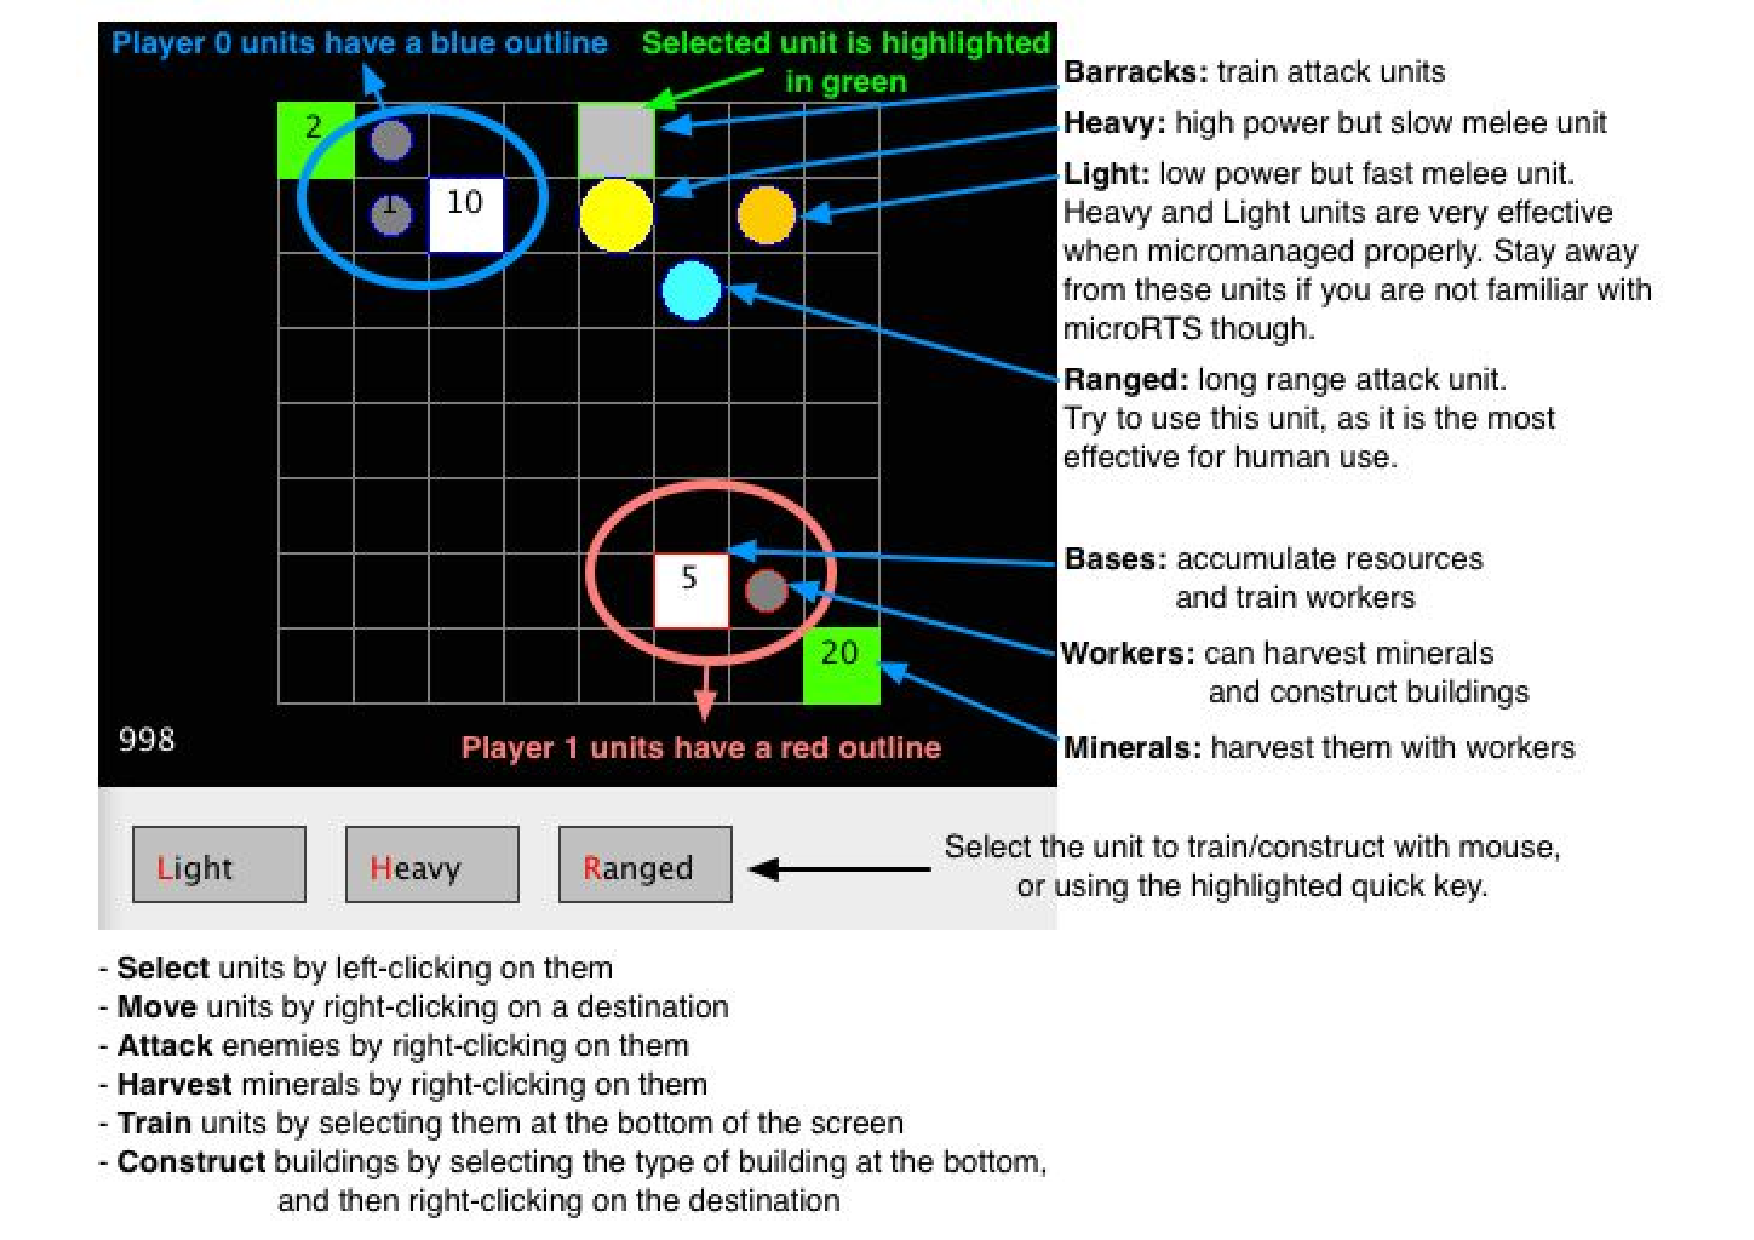
\includegraphics[width=1\textwidth]{fig/microrts.pdf}
	\caption{Uma foto da tela do MicroRTS}
	\label{fig:microrts}
\end{figure} 

No ambiente há algumas estrategias implementados, cada estrategia possui variações dos algoritmos. Algumas estrategias são:
\begin{itemize}
	\item Minimax Alpha-Beta Search Strategies
	\item Monte Carlo Search Strategies
\end{itemize}
